\documentclass[14pt]{beamer}
\usepackage[utf8]{inputenc}
\usepackage[T1]{fontenc}
\usepackage{lmodern}
\usetheme{Ilmenau}
\begin{document}
	\author{Antonio Allocca}
	\title{IKEv2 con Post Quantum Resilience}
	\subtitle{Hardening e proposte alternative}
	\logo{
\includegraphics[height=1cm]{images/logo.png}}
	\institute{Team Cifrante}
	\date{\today}
	\subject{PQC}
	%\setbeamercovered{transparent}
	%\setbeamertemplate{navigation symbols}{}
	\begin{frame}[plain]
		\maketitle
	\end{frame}
	
	\begin{frame}
		\frametitle{\textbf{SIGMA}}
		Aproccio \textit{SIGn-and-MAc} per rendere \textit{DH} \textbf{autenticato}.
		\begin{itemize}
			\item Perfect forward secrecy (PFS)
			\item Scambio di chiavi crittografico
			\item Consistenza tra le comunicazioni
		\end{itemize}
	\end{frame}
	
	\begin{frame}
		\frametitle{\textbf{SIGMA}}
		Disaccoppia l’autenticazione (\textbf{firma} sui valori \textit{DH}) dal binding \textit{chiave-identità} (\textbf{MAC} sulla propria identità).
		
		\center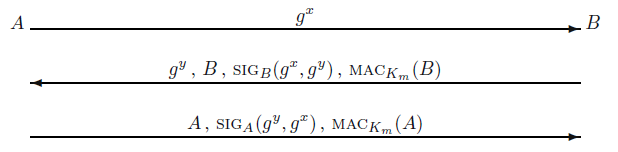
\includegraphics[height=2.5cm]{images/sigma.png}
	\end{frame}
	
	\begin{frame}
		\frametitle{\textbf{SIGMA-R}}
		L'implementazione è simile al \textit{SIGMA} di base, però \textit{B} (il Responder) ritarda l'invio dell'identità ed informazioni di autenticazione finché \textit{A} non gli invia le informazioni di \textit{identità} ed informazioni di \textit{autenticazione}.
		
		\center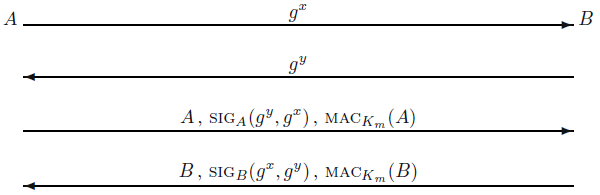
\includegraphics[height=2.5cm]{images/sigma-r.png}
	\end{frame}
	
	\begin{frame}
		\frametitle{\textbf{IKEv2} (\textit{RFC 7296})}
		E' un componente di IPSec.
		
		\textbf{A cosa serve}
		\begin{itemize}
			\item Mutua autenticazione tra i nodi
			\item Stabilire e mantenere le Security Associations (\textbf{SA})
			\begin{itemize}
				\item Encapsulating Security Payload (\textbf{ESP}).
				\item Authentication Header (\textbf{AH}).
				\item Contengono anche l'insieme di \textbf{algoritmi crittografici} che devono essere utilizzati dalle \textit{SA} per \textbf{proteggere} il traffico che trasportano.
			\end{itemize}
		\end{itemize}
	\end{frame}
	
	\begin{frame}
		\frametitle{\textbf{IKEv2} (\textit{RFC 7296})}
		\textbf{Come funziona}
		\begin{itemize}
			\item IKE autentica i nodi e stabilisce le IKE SA.
			\begin{itemize}
				\item Qui viene utilizzato  SIGMA per il KE.
				\item In IKEv2 viene utilizzato SIGMA-R.
			\end{itemize}
			\item Una volta stabilita, la IKE SA crea e fa il rekey delle Child SA tramite CREATE\_CHILD\_SA, senza ripetere l’autenticazione con firme e certificati.
			\item Gli algoritmi usati e stabiliti nelle \textit{SA} vengono proposti dall'initiator.
		\end{itemize}

	\end{frame}
	
	\begin{frame}
		\frametitle{Proposte}
		\begin{itemize}
			\item Implementare la \textbf{frammentazione} dei pacchetti. 
			\item \textbf{Cifrare} dopo lo scambio \textit{DH}. 
			\item \textbf{Rimuovere} autenticazione \textit{DH} ed utilizzare \textit{ML-KEM}.
			\item \textbf{Ibridazione} \textit{DH} ed \textit{ML-KEM}.
		\end{itemize}
	\end{frame}
	
	\begin{frame}
	\frametitle{Implementare la \textbf{frammentazione} dei pacchetti}
	La cifratura \textit{post quantum} utilizza chiavi molto lunghe.
	
	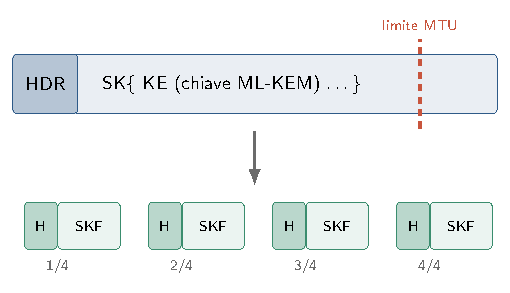
\includegraphics[width=0.75\textwidth]{images/frammentazione.pdf}
	\end{frame}
	
	\begin{frame}
	\frametitle{\textbf{Cifrare} dopo lo scambio \textit{DH}}
	L'autenticazione segue la \textit{crittografia classica}, le chiavi sono incapsulate con \textit{ML-KEM}.
	
	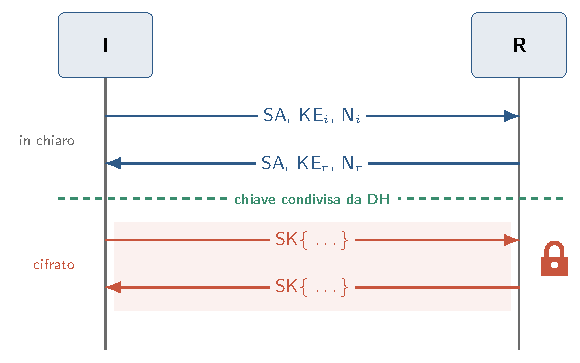
\includegraphics[width=0.75\textwidth]{images/cifratura.pdf}
	\end{frame}
	
	\begin{frame}
	\frametitle{\textbf{Rimuovere} autenticazione \textit{DH} ed utilizzare \textit{ML-KEM}}
	Utilizzo di $KeyGen \to ek \to Encaps \to ct \to Decaps$ con \textit{PSK}.
	
	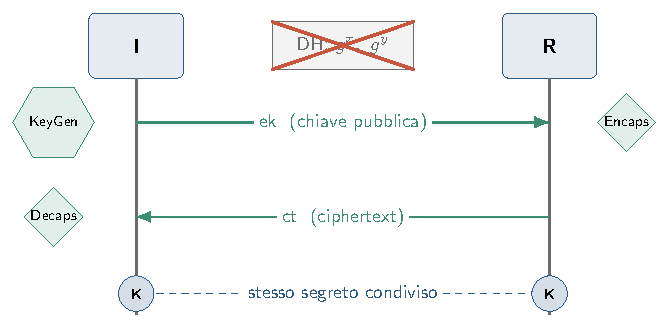
\includegraphics[width=0.75\textwidth]{images/mlkem.pdf}
	\end{frame}
	
	\begin{frame}
	\frametitle{\textbf{Ibridazione} \textit{DH} ed \textit{ML-KEM}}
	il segreto \textit{DH} e quello \textit{ML-KEM} entrano in una \textit{KDF} che produce la chiave di sessione.
	
	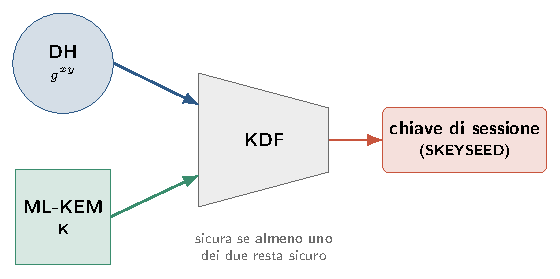
\includegraphics[width=0.75\textwidth]{images/ibrido.pdf}
	\end{frame}
	
\end{document}